%%%%%%%%%%%%%%%%%%%%%%%%%%%%%%%%%%%%%%%%%
% Beamer Presentation
% LaTeX Template
% Version 1.0 (10/11/12)
%
% This template has been downloaded from:
% http://www.LaTeXTemplates.com
%
% License:
% CC BY-NC-SA 3.0 (http://creativecommons.org/licenses/by-nc-sa/3.0/)
%
%%%%%%%%%%%%%%%%%%%%%%%%%%%%%%%%%%%%%%%%%

%----------------------------------------------------------------------------------------
%	PACKAGES AND THEMES
%----------------------------------------------------------------------------------------

\documentclass{beamer}

\mode<presentation> {

% The Beamer class comes with a number of default slide themes
% which change the colors and layouts of slides. Below this is a list
% of all the themes, uncomment each in turn to see what they look like.

%\usetheme{default}
%\usetheme{AnnArbor}
%\usetheme{Antibes}
%\usetheme{Bergen}
%\usetheme{Berkeley}
%\usetheme{Berlin}
%\usetheme{Boadilla}
%\usetheme{CambridgeUS}
%\usetheme{Copenhagen}
%\usetheme{Darmstadt}
%\usetheme{Dresden}
%\usetheme{Frankfurt}
%\usetheme{Goettingen}
%\usetheme{Hannover}
%\usetheme{Ilmenau}
%\usetheme{JuanLesPins}
\usetheme{Luebeck}
%\usetheme{Madrid}
%\usetheme{Malmoe}
%\usetheme{Marburg}
%\usetheme{Montpellier}
%\usetheme{PaloAlto}
%\usetheme{Pittsburgh}
%\usetheme{Rochester} %% Talvez - Colocar logo utfpr
%\usetheme{Singapore} %% Interessante
%\usetheme{Szeged}
%\usetheme{Warsaw}

% As well as themes, the Beamer class has a number of color themes
% for any slide theme. Uncomment each of these in turn to see how it
% changes the colors of your current slide theme.

%\usecolortheme{albatross}
%\usecolortheme{beaver}
%\usecolortheme{beetle}
%\usecolortheme{crane}
%\usecolortheme{dolphin}
%\usecolortheme{dove}
%\usecolortheme{fly}
%\usecolortheme{lily}
\usecolortheme{orchid}
%\usecolortheme{rose}
%\usecolortheme{seagull}
%\usecolortheme{seahorse}
%\usecolortheme{whale}
%\usecolortheme{wolverine}

%\setbeamertemplate{footline} % To remove the footer line in all slides uncomment this line
%\setbeamertemplate{footline}[page number] % To replace the footer line in all slides with a simple slide count uncomment this line

%\setbeamertemplate{navigation symbols}{} % To remove the navigation symbols from the bottom of all slides uncomment this line
}

\setbeamertemplate{caption}[numbered] %% Numbered figures on the project
\setbeamertemplate{headline}{} % Remove header from the title
\usepackage{graphicx} % Allows including images
\usepackage{booktabs} % Allows the use of \toprule, \midrule and \bottomrule in tables
\usepackage{caption}

\usepackage[brazil]{babel}
\usepackage[utf8]{inputenc}

%----------------------------------------------------------------------------------------
%	TITLE PAGE
%----------------------------------------------------------------------------------------

\title[Projeto e implementação de robô seguidor de linha]{Projeto e implementação de \\robô autônomo seguidor de linha} % The short title appears at the bottom of every slide, the full title is only on the title page

\author{\bf Willian Americano Lopes} % Your name
%\small walopes23@gmail.com
\institute[UTFPR] % Your institution as it will appear on the bottom of every slide, may be shorthand to save space
{
Universidade Tecnológica Federal do Paraná - Câmpus Pato Branco\\ % Your institution for the title page
DAINF - Departamento Acadêmico de Informática
\newline

%% NOVO %%
\medskip
Orientador: Professor Fábio Favarim\\
Co-orientador: Professor César Rafael claure Torrico\newline

\medskip
walopes23@gmail.com\\
\{favarim,torrico\} @utfpr.edu.br
}


%\small \date{\today} % Date, can be changed to a custom date
\tiny \date{05 de dezembro de 2017} % Date, can be changed to a custom date

\titlegraphic{}

\begin{document}

%%%%%%%%%%%%%%%%%%%%%%%%%%% LOGO UTFPR  
{
\setbeamertemplate{background}{%
  \raisebox{-0.65cm}{%
    \parbox[c]{3.5cm}{\centering%
      
\includegraphics[width=2cm]{Figuras/utf.pdf}%
    }%
    \parbox[c]{\dimexpr\paperwidth-5.2cm\relax}{\centering%
      {\large Universidade Tecnológica Federal do Paraná}%
    }%
  }%
}    
%%%%%%%%%%%%%%%%%%%%%%%%%%%%%%%%%%%%%%%%

%%%%%%%%%%%%%%%%%%%%%%%%%%%%%%%%%%%% PAGE NUMBER
 \addtobeamertemplate{navigation symbols}{}{%
    \usebeamerfont{footline}%
    \usebeamercolor[fg]{footline}%
    \hspace{1em}%
    \insertframenumber/\inserttotalframenumber
}
%%%%%%%%%%%%%%%%%%%%%%%%%%%%%%%%%%%%%%%%%



\begin{frame}[label=firstframe]
\titlepage % Print the title page as the first slide
\end{frame}

\begin{frame}

\frametitle{Sumário} % Table of contents slide, comment this block out to remove it
\tableofcontents % Throughout your presentation, if you choose to use \section{} and \subsection{} commands, these will automatically be printed on this slide as an overview of your presentation

\end{frame}

%----------------------------------------------------------------------------------------
%	PRESENTATION SLIDES
%----------------------------------------------------------------------------------------

\section{Introdução} % Sections can be created in order to organize your presentation into discrete blocks, all sections and subsections are automatically printed in the table of contents as an overview of the talk
%------------------------------------------------

%\subsection{Robótica} % A subsection can be created just before a set of slides with a common theme to further break down your presentation into chunks

\begin{frame}
\frametitle{Robótica}
Sed iaculis dapibus gravida. Morbi sed tortor erat, nec interdum arcu. Sed id lorem lectus. Quisque viverra augue id sem ornare non aliquam nibh tristique. Aenean in ligula nisl. Nulla sed tellus ipsum. Donec vestibulum ligula non lorem vulputate fermentum accumsan neque mollis.\\~\\

Sed diam enim, sagittis nec condimentum sit amet, ullamcorper sit amet libero. Aliquam vel dui orci, a porta odio. Nullam id suscipit ipsum. Aenean lobortis commodo sem, ut commodo leo gravida vitae. Pellentesque vehicula ante iaculis arcu pretium rutrum eget sit amet purus. Integer ornare nulla quis neque ultrices lobortis. Vestibulum ultrices tincidunt libero, quis commodo erat ullamcorper id.
\end{frame}

%------------------------------------------------

\begin{frame}
\frametitle{Bullet Points}
\begin{itemize}
\item Lorem ipsum dolor sit amet, consectetur adipiscing elit
\item Aliquam blandit faucibus nisi, sit amet dapibus enim tempus eu
\item Nulla commodo, erat quis gravida posuere, elit lacus lobortis est, quis porttitor odio mauris at libero
\item Nam cursus est eget velit posuere pellentesque
\item Vestibulum faucibus velit a augue condimentum quis convallis nulla gravida
\end{itemize}
\end{frame}

%------------------------------------------------

\begin{frame}
\frametitle{Blocks of Highlighted Text}
\begin{block}{Block 1}
Lorem ipsum dolor sit amet, consectetur adipiscing elit. Integer lectus nisl, ultricies in feugiat rutrum, porttitor sit amet augue. Aliquam ut tortor mauris. Sed volutpat ante purus, quis accumsan dolor.
\end{block}

\begin{block}{Block 2}
Pellentesque sed tellus purus. Class aptent taciti sociosqu ad litora torquent per conubia nostra, per inceptos himenaeos. Vestibulum quis magna at risus dictum tempor eu vitae velit.
\end{block}

\begin{block}{Block 3}
Suspendisse tincidunt sagittis gravida. Curabitur condimentum, enim sed venenatis rutrum, ipsum neque consectetur orci, sed blandit justo nisi ac lacus.
\end{block}
\end{frame}

%------------------------------------------------

\begin{frame}
\frametitle{Multiple Columns}
\begin{columns}[c] % The "c" option specifies centered vertical alignment while the "t" option is used for top vertical alignment

\column{.45\textwidth} % Left column and width
\textbf{Heading}
\begin{enumerate}
\item Statement
\item Explanation
\item Example
\end{enumerate}

\column{.5\textwidth} % Right column and width
Lorem ipsum dolor sit amet, consectetur adipiscing elit. Integer lectus nisl, ultricies in feugiat rutrum, porttitor sit amet augue. Aliquam ut tortor mauris. Sed volutpat ante purus, quis accumsan dolor.

\end{columns}
\end{frame}

%%%%%%%%%%%%%%%%%%%%%%% EOF %%%%%%%%%%%%%%%%%%%%%%%%%%%%


%------------------------------------------------
\section{Desenho e implementação}
%------------------------------------------------

%%%%%%%%%%%%%%%%%%%%%%%%%%%%%%%%%%%%%%%%%%%%%%%%%%%%%%%%%%%
%%%%%%%%%%%%%%%%%%%%%%%%%%%%%%%%%%%%%%%%%%%%%%%%%%%%%%%%%%%
\subsection{Projeto do \textit{hardware}}

\begin{frame}
\frametitle{Desenho e implementação}

Projeto do \textit{Hardware}

\begin{figure}[th]
	\centering
	\captionsetup{width=0.65\textwidth,font=footnotesize,textfont=bf}
	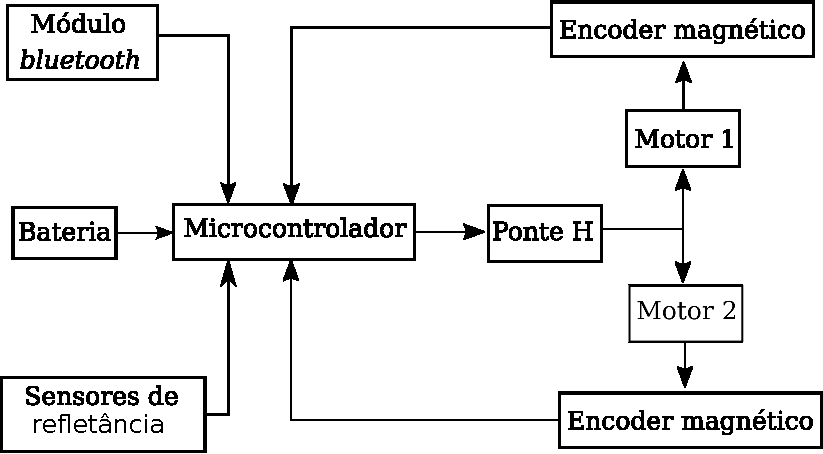
\includegraphics[width=0.65\textwidth,keepaspectratio]{Figuras/DiagramaHW.pdf}
	\caption{Diagrama de funcionamento do \textit{hardware} do veículo.\label{fig:diagEl}}
\end{figure}

\end{frame}

%% ----------------------------------------------------

\begin{frame}
\frametitle{Sensores e condicionamento de sinais}

\begin{figure}[th]
	\centering
	\captionsetup{width=0.65\textwidth,font=footnotesize,textfont=bf}
	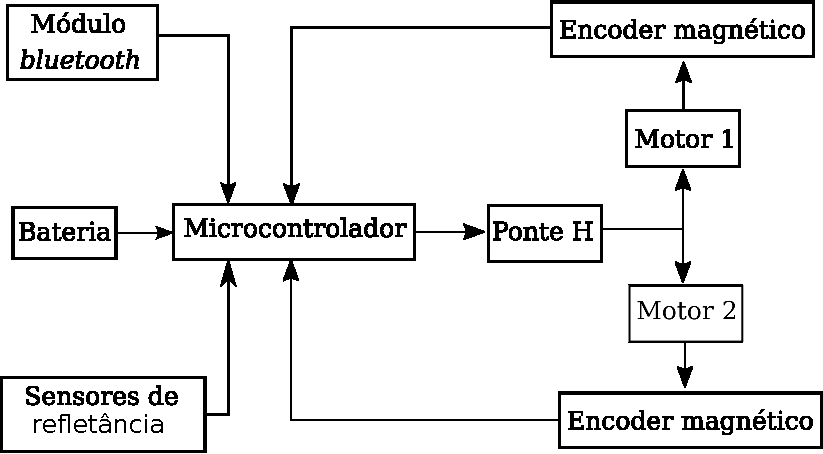
\includegraphics[width=0.65\textwidth,keepaspectratio]{Figuras/DiagramaHW.pdf}
	\caption{Diagrama de funcionamento do \textit{hardware} do veículo.\label{fig:diagEl}}
\end{figure}


\end{frame}

%% To not change the number page of this slide
\begin{frame}[noframenumbering]
\frametitle{Sensores e condicionamento de sinais}



    \transglitter
    \frametitle{Test}
        \begin{itemize}
            \item One
            \item Two
            \item Three
        \end{itemize}
\end{frame}

%% ------------------------------------------------------

\begin{frame}
\frametitle{Sensor de refletância QRE1113}

\begin{figure}[th]
	\centering
	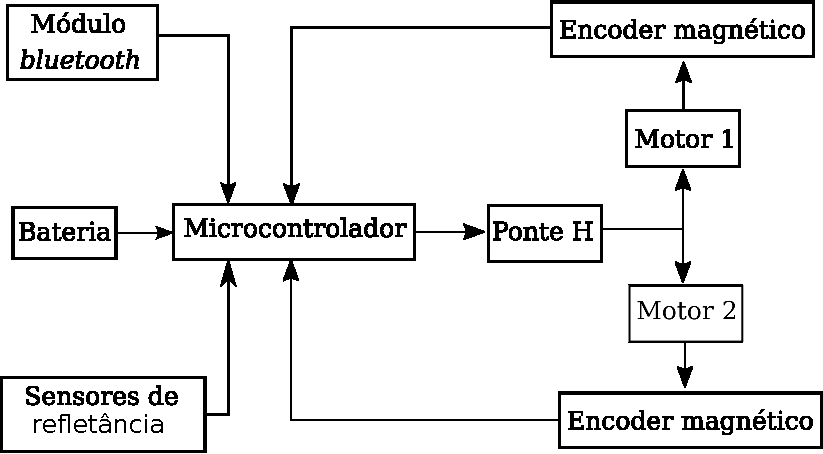
\includegraphics[width=0.65\textwidth,keepaspectratio]{Figuras/DiagramaHW.pdf}
	\caption{Diagrama de funcionamento do \textit{hardware} do veículo.\label{fig:diagEl}}
\end{figure}
\end{frame}

%% ------------------------------------------------------

\begin{frame}
\frametitle{\textit{Driver} de acionamento TB6612FNG}

\begin{figure}[th]
	\centering
	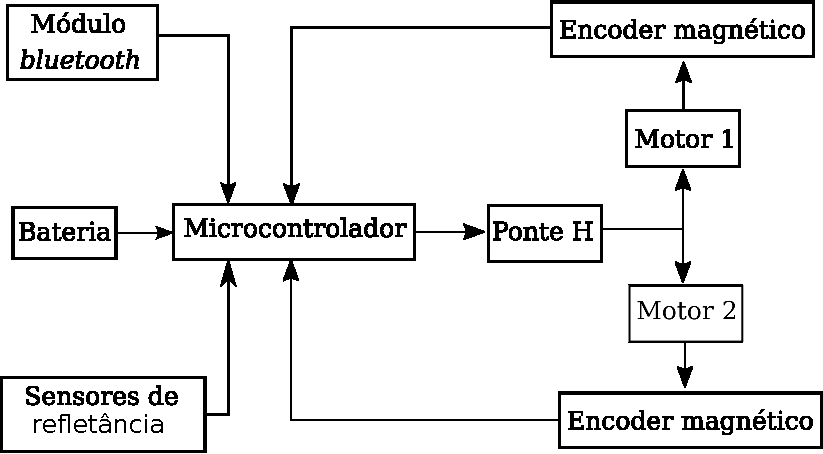
\includegraphics[width=0.65\textwidth,keepaspectratio]{Figuras/DiagramaHW.pdf}
	\caption{Diagrama de funcionamento do \textit{hardware} do veículo.\label{fig:diagEl}}
\end{figure}
\end{frame}

%% ------------------------------------------------------



%%%%%%%%%%%%%%%%%%%%%%%%%%%%%%%%%%%%%%%%%%%%%%%%%%%%%%%%%%%
%%%%%%%%%%%%%%%%%%%%%%%%%%%%%%%%%%%%%%%%%%%%%%%%%%%%%%%%%%%
\subsection{Projeto do controlador de SED}

\begin{frame}
\frametitle{Projeto do controlador de SED}
\begin{columns}
	\column{0.4\linewidth}
		\begin{itemize}
		\item Modelado pelos \textit{softwares} Supremica e Deslab
		\item Autômato de Moore
		\item Variáveis mapeadas:
			\begin{itemize}
			\item B1 (botão);
			\item AcharDir;
			\item PerdeDir;
			\item AchaEsq;
			\item PerdeEsq.
			\end{itemize}
		\end{itemize}
	\column{0.7\linewidth}
		\begin{figure}[th]
		\centering
		\captionsetup{width=\textwidth,font=footnotesize,textfont=bf}
		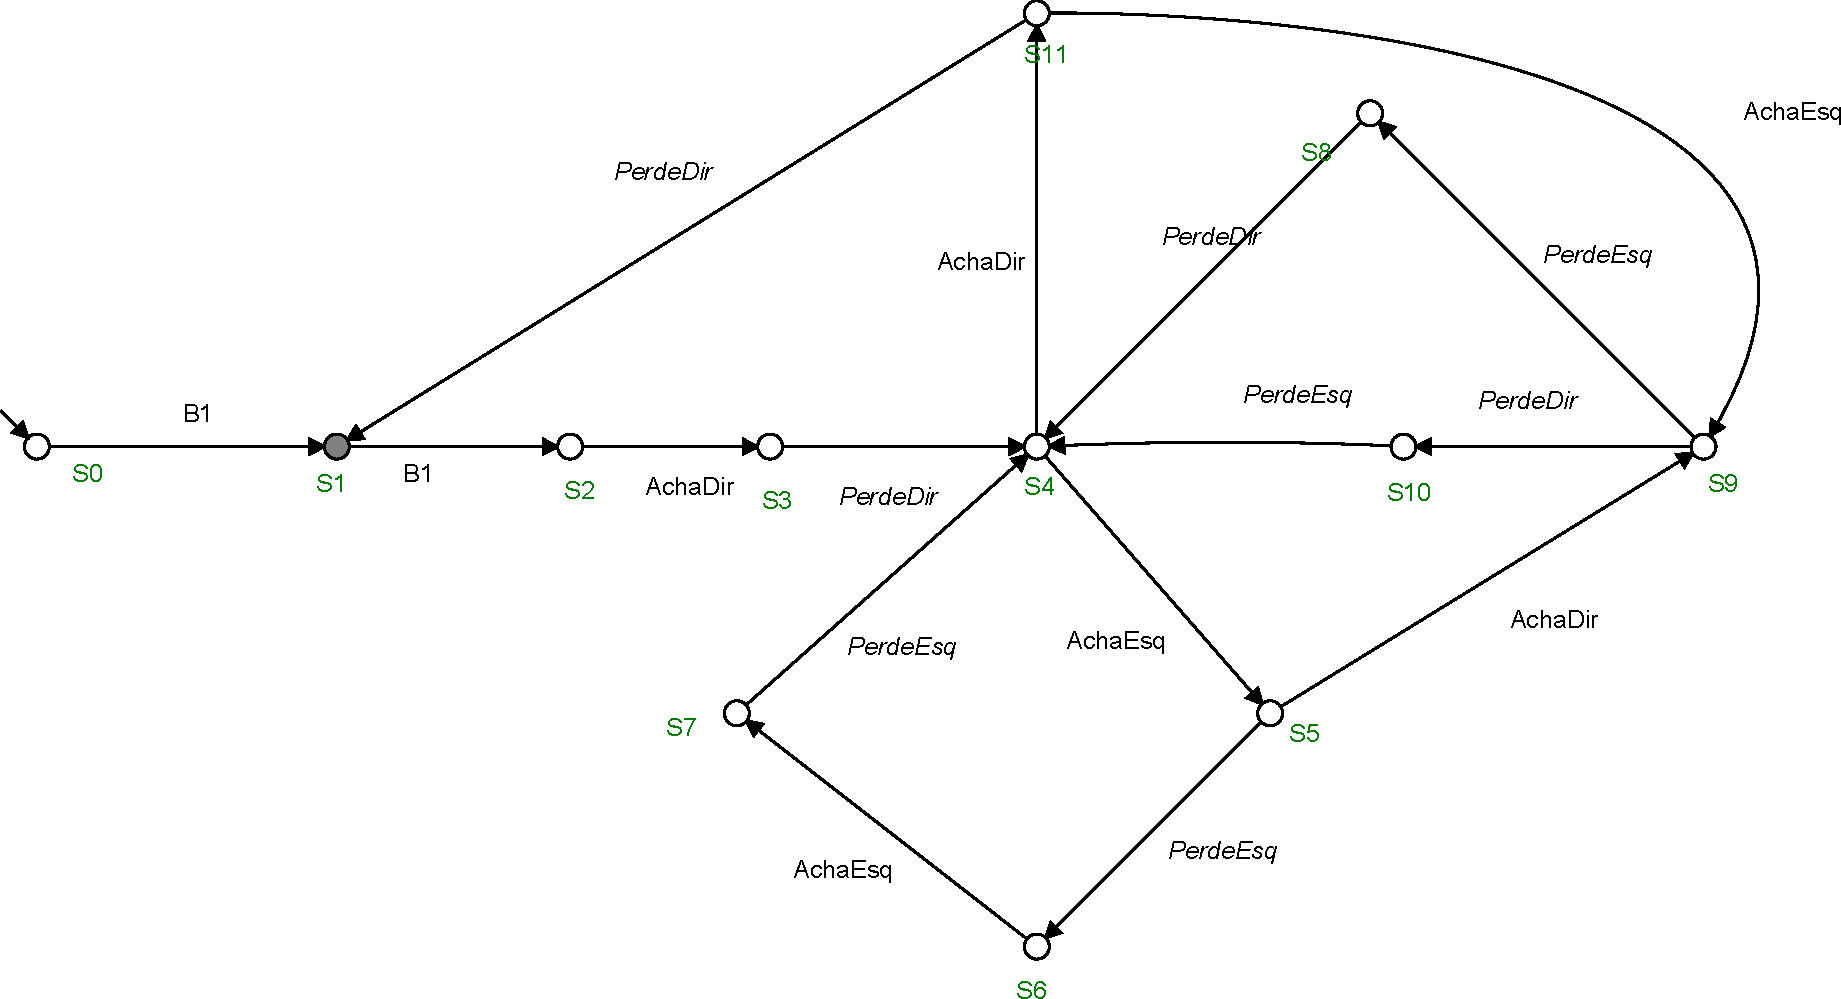
\includegraphics[width=\textwidth,keepaspectratio]{Figuras/SED.pdf}
		\caption{Controlador de SED}				
		\end{figure}
\end{columns}

\end{frame}

%%%%%%%%%%%%%%%%%%%%%%%%%%%%%%%%%%%%%%%%%%%%%%%%%%%%%%%%%%%
%%%%%%%%%%%%%%%%%%%%%%%%%%%%%%%%%%%%%%%%%%%%%%%%%%%%%%%%%%%
\subsection{Projeto do sistema de mapeamento}

\begin{frame}
\frametitle{Projeto do sistema de mapeamento}
\begin{columns}
	\column{0.4\linewidth}
		\begin{itemize}
		\item Armazenamento na memória \textit{flash}
		\item Contém as seguintes informações:
			\begin{itemize}
			\item Quantidade de marcações;
			\item Início e fim de marcação da direita;
			\item Início e fim de marcação da esquerda;
			\end{itemize}
		\end{itemize}
	\column{0.7\linewidth}
		\begin{figure}[th]
		\centering
		\captionsetup{width=\textwidth,font=footnotesize,textfont=bf}
		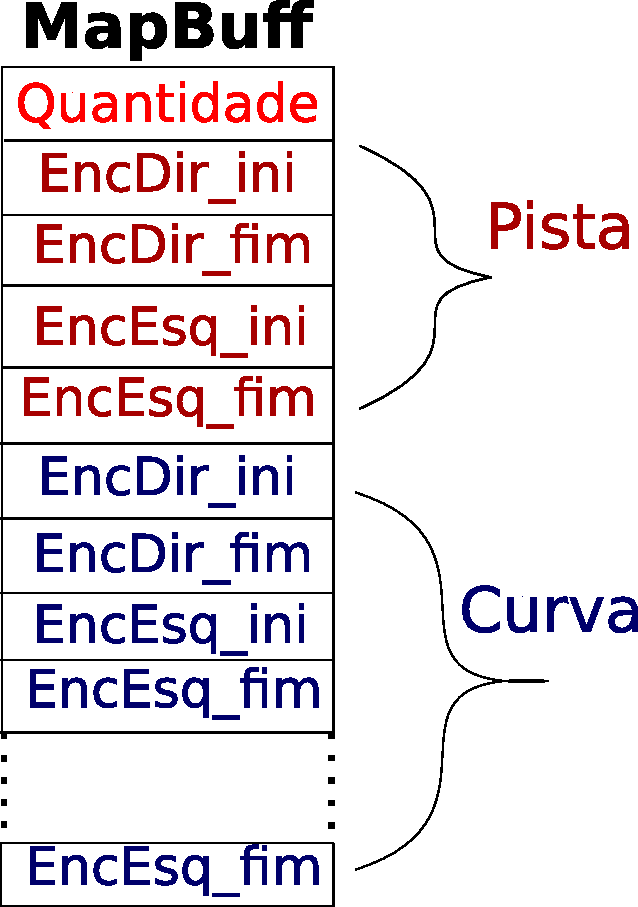
\includegraphics[width=0.6\linewidth,keepaspectratio]{Figuras/VetorMap.pdf}
		\caption{Vetor de armazenamento na \textit{flash}}				
		\end{figure}
\end{columns}

\end{frame}

%%%%%%%%%%%%%%%%%%%%%%%%%%%%%%%%%%%%%%%%%%%%%%%%%%%%%%%%%%%
%%%%%%%%%%%%%%%%%%%%%%%%%%%%%%%%%%%%%%%%%%%%%%%%%%%%%%%%%%%
\subsection{Função de transferência do veículo}

\begin{frame}
\frametitle{Função de Transferência do veículo}
\textbf{Aquisição dos valores da planta}
\begin{columns}
	\column{0.4\linewidth}
		\begin{itemize}
		\item Obtenção da posição
		\item Mesmo PWM para os motores
		\item Motores em sentidos opostos
		\item Informações enviadas via \textit{bluetooth}
		\item É esperado um gráfico próximo a uma rampa
		\end{itemize}
	\column{0.7\linewidth}
		\begin{figure}[th]
		\centering
		\captionsetup{width=\textwidth,font=footnotesize,textfont=bf}
		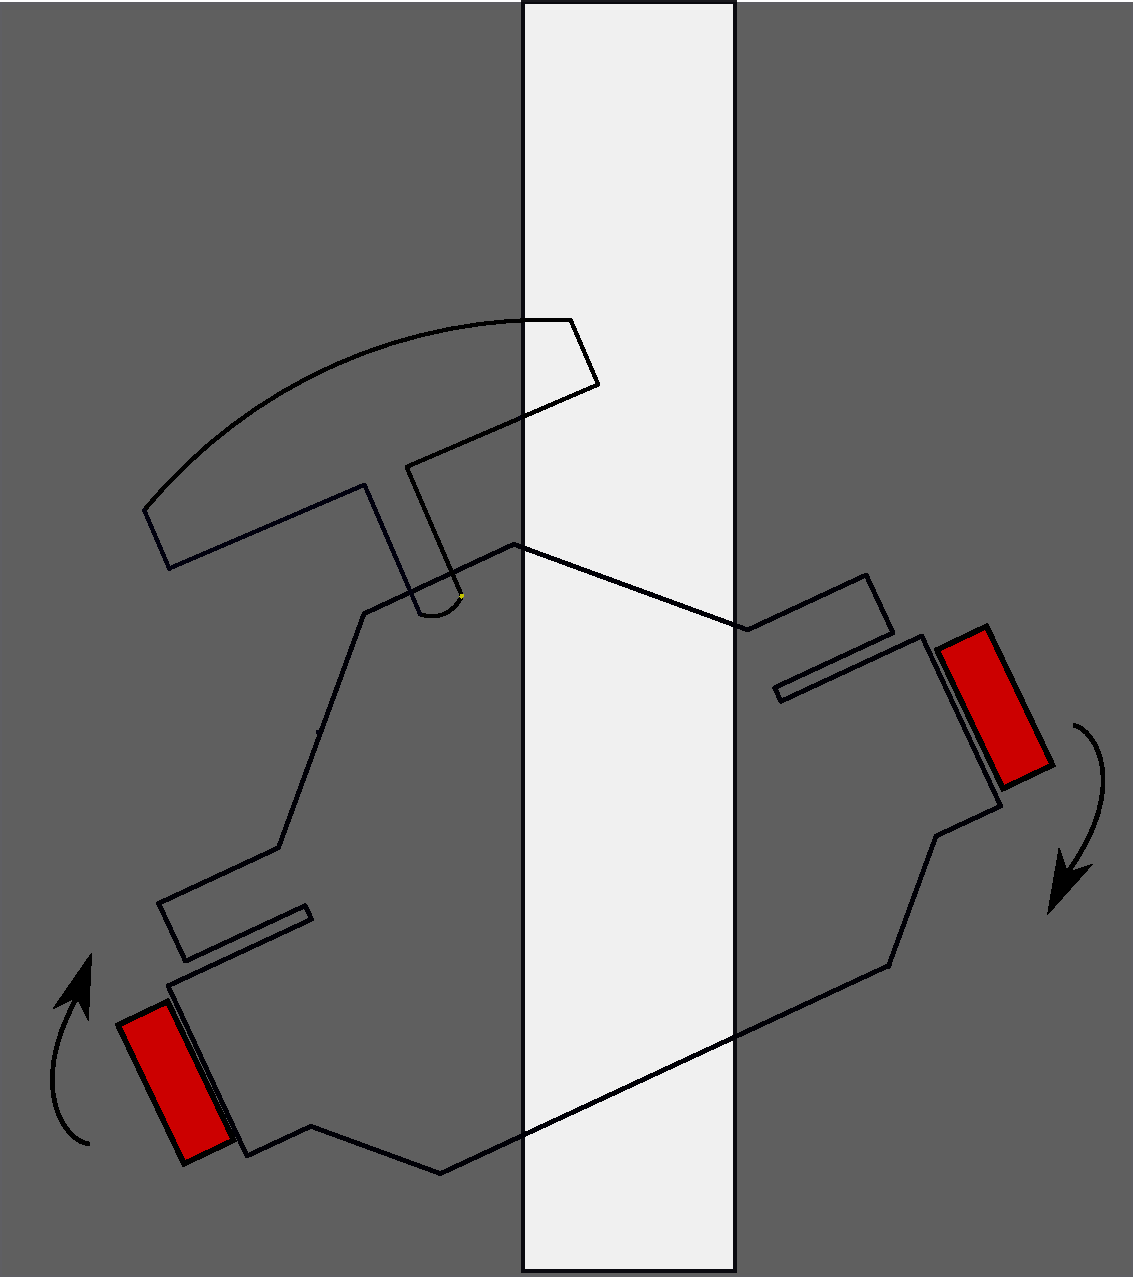
\includegraphics[width=0.6\linewidth,keepaspectratio]{Figuras/FT.pdf}
		\caption{Aquisição dos valores de posição do robô}				
		\end{figure}
\end{columns}
\end{frame}


\begin{frame}
\frametitle{Função de Transferência do veículo}
\textbf{Modelo da função de transferência}\\
	Para encontrar a velocidade, deriva-se a posição
	
\begin{columns}
	\column{0.5\linewidth}

	\begin{figure}[th]
	\centering
	\captionsetup{width=\textwidth,font=footnotesize,textfont=bf}
	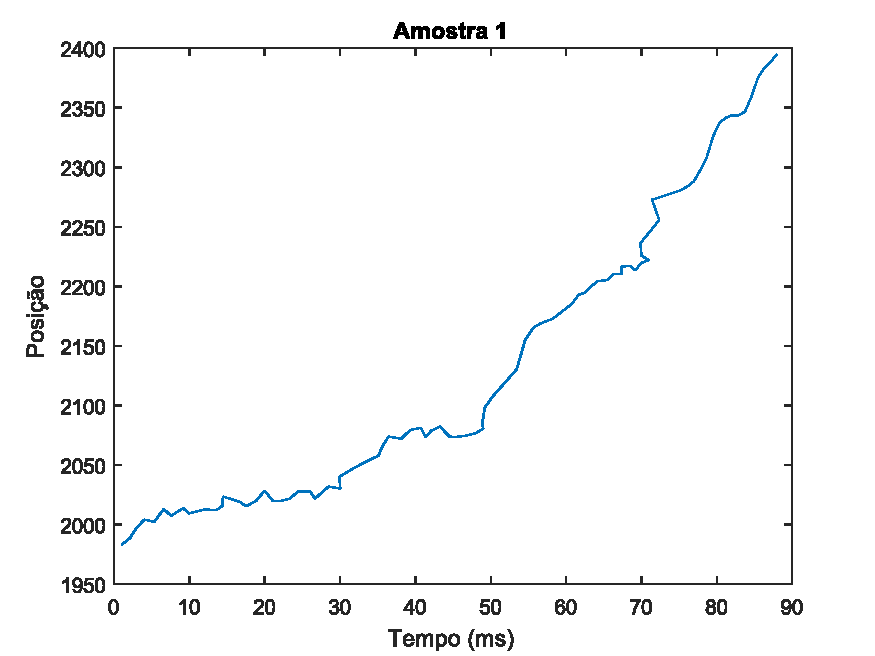
\includegraphics[width=\linewidth,keepaspectratio]{Figuras/Posicao3v2.pdf}
	\caption{Gráfico da posição obtida}				
	\end{figure}
 	
	%\pause 	
 	\column{0.5\linewidth}
	\begin{figure}[th]
	\centering
	\captionsetup{width=\textwidth,font=footnotesize,textfont=bf}
	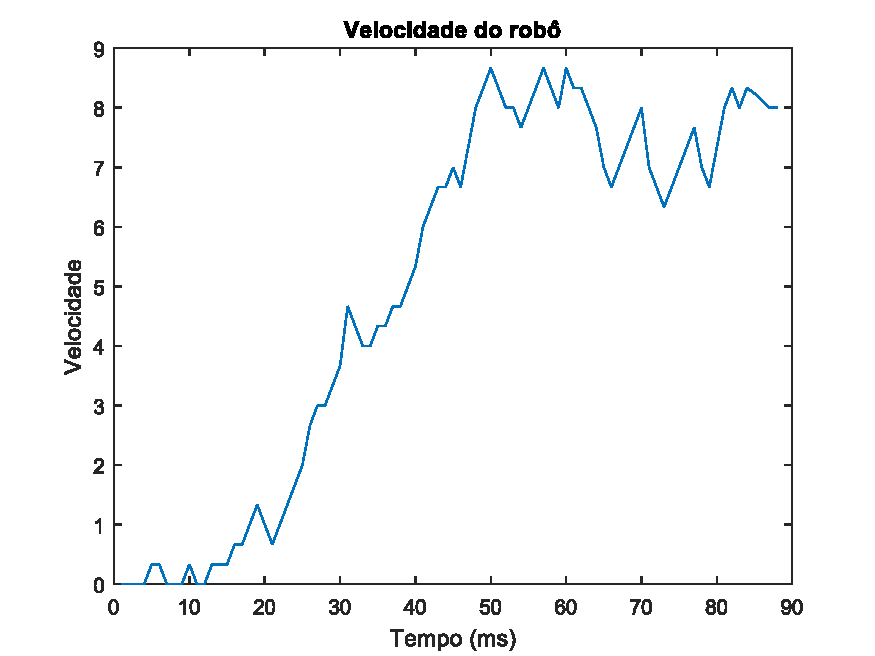
\includegraphics[width=\linewidth,keepaspectratio]{Figuras/Derivadav2.pdf}
	\caption{Gráfico da velocidade}				
	\end{figure}
\end{columns}
\end{frame}



\begin{frame}
\frametitle{Função de Transferência do veículo}
\textbf{Modelo da função de transferência}\\
Com o Matlab, verificou-se uma função que mais se aproxima da desejada
	
\begin{columns}
 		
 	\column{0.45\linewidth}
 	\vspace{-0.5cm}
 	\begin{itemize}
 	\item $P2ZU = 0,0054915(\frac{1-0,011087s}{1+0,014889s+0,000238s^2})$
 	\item A função contém 3 polos e 1 zero
 	\end{itemize}
 	
 	\column{0.55\linewidth}

	\begin{figure}[th]
	\centering
	\captionsetup{width=0.9\textwidth,font=footnotesize,textfont=bf}
	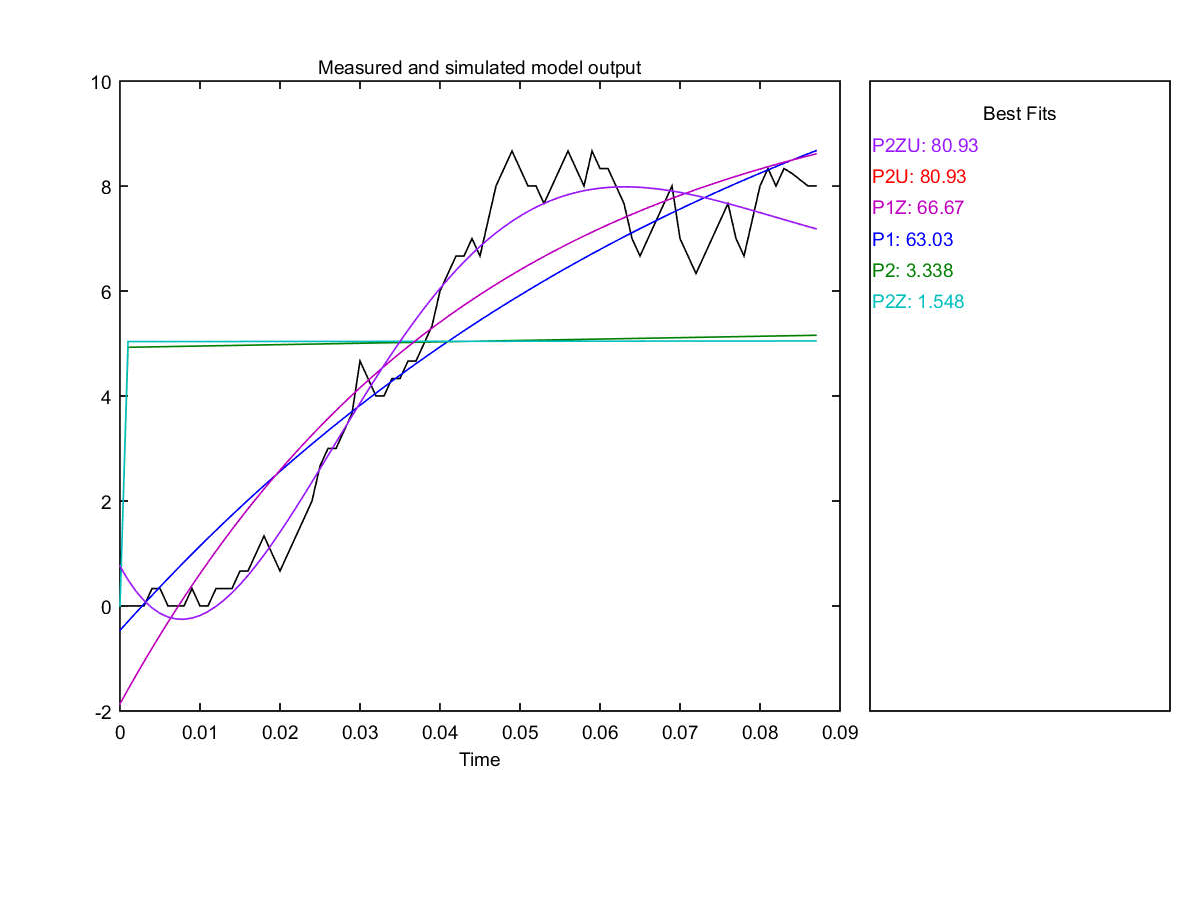
\includegraphics[width=\linewidth,keepaspectratio]{Figuras/Comparativo.pdf}
	\caption{Comparativo feito pelo System Identification}				
	\end{figure}
	
\end{columns}
\end{frame}

\begin{frame}
\frametitle{Função de Transferência do veículo}
\textbf{Modelo da função de transferência}\\
	
\begin{columns}

	\column{0.5\linewidth}
 	\begin{itemize}
 	\item A função encontrada é relacionada à velocidade
 	\item Para a original, é necessário integrá-la e multiplicá-la pelo ganho
 	\item $FT: 1223(\frac{P2Z2}{s})$
	\end{itemize} 		

 	\column{0.5\linewidth}
	\begin{figure}[th]
	\centering
	\captionsetup{width=0.85\textwidth,font=footnotesize,textfont=bf}
	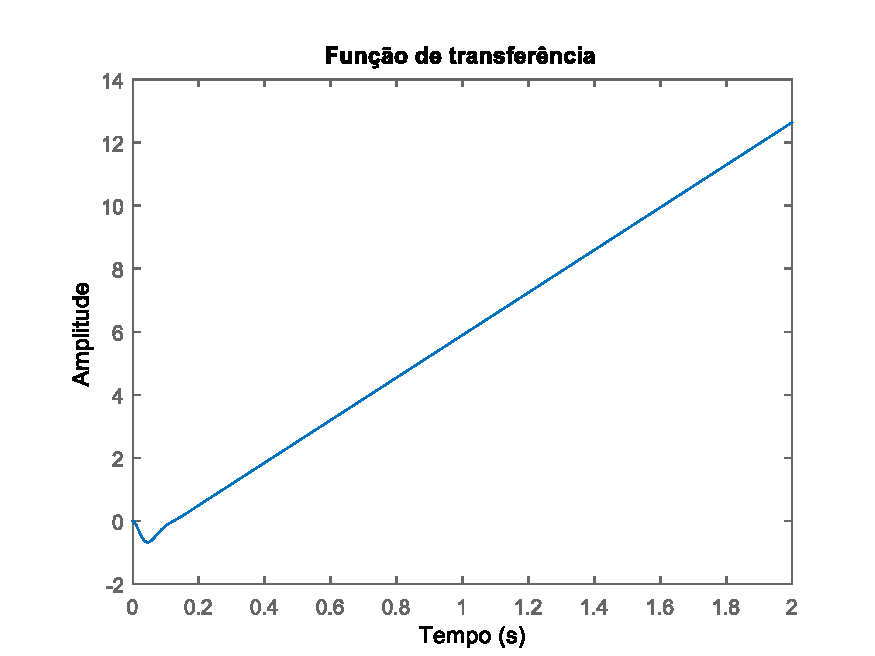
\includegraphics[width=\linewidth,keepaspectratio]{Figuras/planta2v2.pdf}
	\caption{Função de transferência encontrada}				
	\end{figure}
	
\end{columns}
\end{frame}

%%%%%%%%%%%%%%%%%%%%%%%%%%%%%%%%%%%%%%%%%%%%%%%%%%%%%%%%%%%
%%%%%%%%%%%%%%%%%%%%%%%%%%%%%%%%%%%%%%%%%%%%%%%%%%%%%%%%%%%
\subsection{Projeto do controlador de tempo contínuo}


\begin{frame}
\frametitle{Projeto do controlador de tempo contínuo}

\begin{itemize}
\item Controlador Proporcional-Derivativo (PD)
\item Variável controlada é a posição
\end{itemize}

\begin{equation}\label{eq:posicao}
posicao = \frac{\sum_{n=1}^{5} 1000(n-1)V_{n}}{\sum_{n=1}^{5} V_{n}}
\end{equation}

\begin{equation}\label{eq:posicao2}
posicao = \frac{0*V_{1} + 1000*V_{2} + 2000*V_{3} + 3000*V_{4} + 4000*V_{5} }{V_{1} + V_{2} + V_{3} + V_{4} + V_{5}}
\end{equation}

\end{frame}

%%% VER PARA TALVEZ COLOCAR O CODIGO DO PD CONTROLLER

%
%\begin{frame}
%\frametitle{Theorem}
%\begin{theorem}[Mass--energy equivalence]
%$E = mc^2$
%\end{theorem}
%\end{frame}


\begin{frame}[fragile] % Need to use the fragile option when verbatim is used in the slide
\frametitle{Verbatim}
\begin{example}[Theorem Slide Code]
\begin{verbatim}
\begin{frame}
\frametitle{Theorem}
\begin{theorem}[Mass--energy equivalence]
$E = mc^2$
\end{theorem}
\end{frame}\end{verbatim}
\end{example}
\end{frame}



%\begin{figure}[H]
%     \centering
%     \captionsetup{width=0.7\textwidth,font=footnotesize,textfont=bf}
%     \begin{subfigure}[b]{\textwidth}
% 	\centering
%         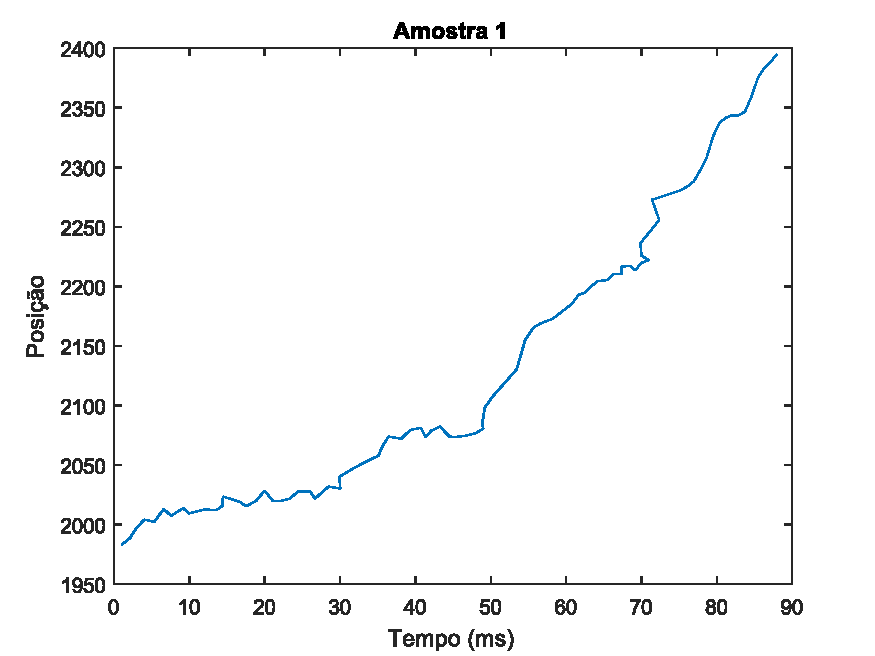
\includegraphics[width=0.6\textwidth,height=\textheight,keepaspectratio]{figuras/Posicao3v2.pdf}
%         \caption{\centering \label{fig:Posicaofinal}}
%     \end{subfigure}
%     
%     \begin{subfigure}[b]{\textwidth}
% 	\centering
%         \includegraphics[width=0.8\textwidth,height=0.3\textheight,keepaspectratio]{figuras/Posicaofinalv2.pdf}
%         \caption{\centering \label{fig:Posicao1}}
%     \end{subfigure}
%
%     \caption{Gráficos da posição em função do tempo (ms), com frequência de 16 KHz e \textit{duty cycle} de 30\%: (a) Amostra 1; (b) Amostra 2 \label{fig:posicoes}}
%     \vspace{-0.3cm}
%     \caption*{Fonte: Autoria própria}
% \end{figure}


%------------------------------------------------



%------------------------------------------------

%% Repeat the title page
\againframe{firstframe}


%----------------------------------------------------------------------------------------

\end{document} 